%!TEX root = ../main.tex
\section{Κατάτμηση εικόνων}

Στην υπολογιστική όραση, με τον όρο κατάτμηση εικόνων αναφερόμαστε στη διαδικασία της διαίρεσης μίας ψηφιακής εικόνας σε πολλαπλά τμήματα (σύνολα εικονοστοιχείων). Ο στόχος της είναι να απλοποιήσει και / ή να αλλάξει την αναπαράσταση της εικόνας σε κάτι πιο ουσιαστικό και ευκολότερο στην ανάλυση. Χρησιμοποιείται κυρίως για τον εντοπισμό αντικειμένων και ορίων (γραμμών, ακμών, κά). Πιο συγκεκριμένα, η κατάτμηση της εικόνας είναι η διαδικασία εκχώρησης μιας ετικέτας σε κάθε εικονοστοιχείο της, έτσι ώστε εικονοστοιχεία με την ίδια ετικέτα να μοιράζονται ορισμένα χαρακτηριστικά.

Στο παρόν κεφάλαιο θα ασχοληθούμε κυρίως με την ανίχνευση ακμών και πιο συγκεκριμένα με τον ανιχνευτή ακμών Canny.

\section{Εισαγωγή στην αναγνώριση ακμών}

Παρόλο που η αναγνώριση σημείων και γραμμών παίζουν σημαντικό ρόλο στην κατάτμηση εικόνων, η αναγνώριση ακμών είναι η πιο συνηθισμένη προσέγγιση για την αναγνώριση σημαντικών ασυνεχειών σε μια εικόνα. Η ανίχνευση ακμών περιλαμβάνει μια ποικιλία μαθηματικών μεθόδων που στοχεύουν στην αναγνώριση σημείων σε μια ψηφιακή εικόνα στην οποία η φωτεινότητά της αλλάζει απότομα ή εμφανίζει ασυνέχειες. Τα σημεία στα οποία αλλάζει έντονα η φωτεινότητα της εικόνας είναι συνήθως οργανωμένα σε ένα σύνολο τμημάτων καμπύλων γραμμών που ορίζονται ως άκρα. Το ίδιο πρόβλημα εντοπισμού ασυνεχειών σε μονοδιάστατα σήματα είναι γνωστό ως ανίχνευση βημάτων και το πρόβλημα της ανεύρεσης ασυνεχειών σήματος με την πάροδο του χρόνου είναι γνωστό ως ανίχνευση αλλαγής. Η ανίχνευση ακμών είναι ένα θεμελιώδες εργαλείο στην επεξεργασία εικόνας, τη μηχανική όραση και την υπολογιστική όραση, ιδιαίτερα στους τομείς της ανίχνευσης χαρακτηριστικών και της εξαγωγής χαρακτηριστικών.

Ο σκοπός της ανίχνευσης αιχμηρών αλλαγών στη φωτεινότητα μιας εικόνας είναι η καταγραφή σημαντικών γεγονότων και αλλαγών στις ιδιότητες του κόσμου. Εύκολα διαπιστώνεται ότι κάτω από γενικές υποθέσεις, οι ασυνέχεις της φωτεινότητας σε μια εικόνα αντιστοιχούν σε:
\begin{itemize}
	\item ασυνέχειες βάθους
	\item ασυνέχειες στον προσανατολισμό της επιφάνειας
	\item αλλαγές στις ιδιότητες των υλικών
	\item μεταβολές στο φωτισμό της σκηνής \\
\end{itemize}
Στην ιδανική περίπτωση, η εφαρμογή ενός ανιχνευτή ακμών μπορεί να οδηγήσει σε ένα σύνολο συνδεδεμένων καμπυλών που υποδεικνύουν τα όρια των αντικειμένων μίας και των επιφανειών μίας εικόνας. Η εφαρμογή ενός τέτοιου αλγορίθμου μειώνει σημαντικά την ποσότητα των προς επεξεργασία δεδομένων και συνεπώς μπορεί να φιλτράρει πληροφορίες που μπορούν να θεωρηθούν λιγότερο σημαντικές, διατηρώντας παράλληλα τις σημαντικές δομικές ιδιότητες της εικόνας. Εάν η διαδικασία της ανίχνευσης ακμών είναι επιτυχής, η ερμηνεία των πληροφοριών της εικόνας απλοποιείται ουσιαστικά. Στην πραγματικότητα όμως, είναι αρκετά δύσκολο να αποκτηθούν ιδανικές ακμές σε εικόνες της καθημερινής ζωής με μέτρια πολυπλοκότητα.

Οι ακμές που εξάγονται από εικόνες με μη σημαντικό περιεχόμενο, συχνά παρεμποδίζονται από κατακερματισμό, δηλαδή ακμές που δεν συνδέονται ώστε να σχηματίσουν τμήματα καμπυλών καθώς και ψευδείς ακμές που δεν αντιστοιχούν σε ενδιαφέροντα σημεία.

Η ανίχνευση ακμών είναι ένα από τα θεμελιώδη βήματα στην επεξεργασία, την ανάλυση και την αναγνώριση προτύπων της εικόνας καθώς και σε τεχνικές υπολογιστικής όρασης. Για το λόγο αυτό, θα ασχοληθούμε με τον αλγόριθμο αναγνώρισης ακμών Canny ο οποίος θα αναλυθεί στη συνέχεια.

\subsection{Προσεγγίσεις}

Υπάρχουν πολλές μέθοδοι ανίχνευσης ακμών, αλλά οι περισσότερες από αυτές μπορούν να ομαδοποιηθούν σε δύο κατηγορίες, βασισμένες σε αναζήτηση και zero-crossing. Οι μέθοδοι που ανήκουν στην πρώτη κατηγορία ανιχνεύουν τις ακμές, υπολογίζοντας πρώτα ένα μέτρο της `δύναμης' της ακμής - συνήθως μια έκφραση της παραγώγου πρώτης τάξης - όπως το μέτρο της κλίσης και στη συνέχεια αναζητώντας τοπικά κατευθυντικά μέγιστα του μέτρου της κλίσης. Οι μέθοδοι της δεύτερης κατηγορίας αναζητούν zero crossings σε παραγώγους δεύτερης τάξης. Συνήθως χρησιμοποιούνται Laplacian zero crossings ή zero crossings μίας μη γραμμικής διαφορικής έκφρασης. Ως στάδιο προκαταρκτικής επεξεργασίας, εφαρμόζεται σχεδόν πάντα ένα στάδιο εξομάλυνσης, συνήθως εξομάλυνση Gaussian για την μείωση του θορύβου.

Οι μέθοδοι ανίχνευσης άκρων που έχουν δημοσιευθεί διαφέρουν κυρίως στους τύπους φίλτρων εξομάλυνσης που εφαρμόζονται και τον τρόπο με τον οποίο υπολογίζονται οι ακμές. Καθώς πολλές μέθοδοι βασίζονται στον υπολογισμό των διαβαθμίσεων της εικόνας, διαφέρουν επίσης και στους τύπους φίλτρων που χρησιμοποιούνται για τον υπολογισμό των εκτιμήσεων κλίσης στις x και y κατευθύνσεις.

\section{Ανιχνευτής ακμών Canny}

Ο ανιχνευτής ακμών Canny είναι ένας αλγόριθμος πολλαπλών σταδίων με στόχο τον υπολογισμό ενός μεγάλου εύρους ακμών σε μία εικόνα. Αναπτύχθηκε από τον John F. Canny \footnote{https:\textbackslash\textbackslash en.wikipedia.org\textbackslash wiki\textbackslash John\_Canny} το 1986 με στόχο να είναι ένας άριστος ανιχνευτής ακμών. Αποτελεί ακόμα μία από τις πιο συνηθισμένες μεθόδους ανίχνευσης ακμών.
\subsection{Ανάπτυξη του αλγορίθμου}

Ο Canny διαπίστωσε ότι οι απαιτήσεις για την εφαρμογή ανίχνευσης ακμών σε διαφορετικά συστήματα όρασης είναι σχετικά παρόμοιες. Επομένως, μια τέτοια λύση μπορεί να εφαρμοστεί σε ένα ευρύ φάσμα καταστάσεων.
\newpage \noindent Τα γενικά κριτήρια ανίχνευσης ακμών περιλαμβάνουν:
\begin{itemize}
	\item Ανίχνευση ακμής με χαμηλό ρυθμό σφάλματος, δηλαδή η ανίχνευση πρέπει να προσδιορίσει με ακρίβεια όσες περισσότερες ακμές μίας εικόνας μπορεί
	\item Το σημείο της ακμής που προσδιορίστηκε να είναι εντοπισμένο με ακρίβεια στο κέντρο της
	\item Μια δεδομένη ακμή της εικόνας θα πρέπει να σημειώνεται μόνο μία φορά και όπου είναι δυνατόν, ο θόρυβος της εικόνας δε πρέπει να δημιουργεί ψευδείς ακμές \\
\end{itemize}

Μεταξύ των μεθόδων ανίχνευσης ακμών που έχουν αναπτυχθεί μέχρι τώρα, ο αλγόριθμος του Canny είναι ένας από τις πιο αυστηρά καθορισμένες μεθόδους, παρέχοντας καλή και αξιόπιστη ανίχνευση. Λόγω της ικανότητάς του να πληροί τις τρεις προϋποθέσεις που αναφέρθηκαν παραπάνω, έγινε ένας από τους πιο δημοφιλείς αλγορίθμους ανίχνευσης ακμών.

\subsection{Διαδικασία ανίχνευσης ακμών}

Η διαδικασία της ανίχνευσης ακμών αναλύεται στα ακόλουθα βήματα:
\begin{enumerate}
   \item Μετατροπή RGB εικόνας σε grayscale
	\item Εφαρμογή Gaussian φίλτρου για τη μείωση του θορύβου της εικόνας και την εξομάλυνσή της
	\item Υπολογισμός του μέτρου της κλίσης και της κατεύθυνσης της
	\item Διαγραφή ακμών που δεν είναι τοπικά μέγιστα (Non-maximum suppression)
	\item Εφαρμογή διπλής κατωφλίωσης για τον καθορισμό πιθανών ακμών
	\item Σύνδεση ακμών με μέθοδο υστέρησης. Ολοκλήρωση της ανίχνευσης των ακμών, αφαιρώντας όλες όσες είναι αδύναμες και δε συνδέονται με ισχυρές ακμές \\
\end{enumerate}
Στη συνέχεια θα αναλυθούν τα προαναφερθέντα στάδια του αλγορίθμου.
\newpage
\begin{itemize}[label={},leftmargin=*]
\item \textbf{Μετατροπή RGB σε grayscale}

Το πρώτο βήμα της διαδικασίας εύρεσης ακμών είναι η μετατροπή της RGB εικόνας σε grayscale. Αυτό γίνεται κυρίως για λόγους πολυπλοκότητας κατά τη διάρκεια της επεξεργασίας και μείωσης του συνολικού όγκου δεδομένων. Η μετατροπή αυτή είναι μία εύκολη διαδικασία και μπορεί να εφαρμοστεί σε εφαρμογές πραγματικού χρόνου.

Ενώ υπάρχουν πολλοί τρόποι για να μετατραπεί η αρχική εικόνα σε grayscale ο πιο συνηθισμένος είναι να ευρεθεί ο μέσος όρος των 3 καναλιών (R,G,B). Η μέθοδος αυτή όμως δεν παράγει ικανοποιητικά αποτελέσματα.
\[Gray = (Red + Green + Blue) / 3\]

H ITU-R\footnote{https:\textbackslash\textbackslash en.wikipedia.org\textbackslash wiki\textbackslash ITU-R} προτείνει τη μέθοδο Luma\footnote{https:\textbackslash\textbackslash en.wikipedia.org\textbackslash wiki\textbackslash Luma\textunderscore (video)}, που είναι ο σταθμισμένος όρος των RGB συνιστωσών ως την καταλληλότερη μέθοδο για μετατροπή σε grayscale. Η μέθοδος αυτή δίνεται από τον ακόλουθο τύπο.
\[Gray = 0.2126\times Red + 0.7152\times Green + 0.00722\times Blue\]
\begin{figure}[H]
   \centering
   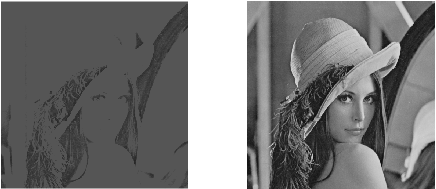
\includegraphics[width=\textwidth]{images/gray}\\
   \caption{Μετατροπή σε grayscale, μέσος όρος \& μέθοδος Luma}
\end{figure}

Είναι εμφανές ότι η μέθοδος του μέσου όρου δε παράγει ικανοποιητικά αποτελέσματα καθώς δε λαμβάνει υπόψη της τα επίπεδα της φωτεινότητας του κάθε καναλιού. \\
\hfill \break
\item \textbf{Gaussian φίλτρο}

Δεδομένου ότι όλα τα αποτελέσματα ανίχνευσης ακμών επηρεάζονται εύκολα από το θόρυβο της εικόνας, είναι απαραίτητο να φιλτραριστεί για να αποτραπεί η ψευδής ανίχνευση ακμών. Για την εξομάλυνση χρησιμοποείται ένα Gaussian φίλτρο. Καθώς, ο μετασχηματισμός Fourier της Gaussian συνάρτησης δίνει άλλη μία Gaussian συνάρτηση, η εφαρμογή του θολώματος μειώνει τα υψηλής συχνότητας στοιχεία μίας εικόνας. Συνεπώς, μπορούμε να θεωρήσουμε το Gaussian blur ώς ένα χαμηλοπερατό φίλτρο.

Το Gaussian blur είναι ένας τύπος φίλτρου θολώματος που χρησιμοποιεί μία συνάρτηση Gaussian (που εκφράζει επίσης την κανονική κατανομή) για να υπολογίσει το μετασχηματισμό του κάθε εικονοστοιχείου της εικόνας. Η εξίσωση για το Gaussian φίλτρο σε δύο διαστάσεις δίνεται από:
\begin{equation}
G(x,y) = \frac{1}{2\pi\sigma^2}e^{-(x^2+y^2)/2\sigma^2}
\end{equation}
όπου $x$  είναι η απόσταση από τη αρχή του οριζόντιου άξονα, $y$ η απόσταση από τη αρχή του κάθετου άξονα και $\sigma$ η τυπική απόκλιση της Gaussian κατανομής. Με την αύξηση της τυπικής απόκλισης επιτυγχάνεται μεγαλύτερο θόλωμα της εικόνας όπως φαίνεται στο σχήμα.

Απαραίτητη προϋπόθεση του φίλτρου είναι ότι το άθροισμα όλων των συντελεστών του πρέπει να ισούται με 1. Επομένως, για την αποφυγή αύξησης της φωτεινότητας της εικόνας πρέπει να κανονικοποιηθεί. Αυτό επιτυγχάνεται μέσω της πρόσθεσης όλων των συντελεστών και της διαίρεσης τους με το άθροισμα αυτό.

\newpage Για παράδειγμα, ένα συμμετρικό φίλτρο μεγέθους $3x3$ και $\sigma=1$ είναι το ακόλουθο:
% https://softwarebydefault.com/2013/06/08/calculating-gaussian-kernels/
\[
	G = \begin{bmatrix}
    0.0751 & 0.1238 & 0.0751  	\\
   	0.1238 & 0.2042 & 0.1238  	\\
    0.0751 & 0.1238 & 0.0751		\\
\end{bmatrix}\quad = \frac{1}{0.7799} \times
\begin{bmatrix}
    0.0586 & 0.0966 & 0.0586     \\
      0.0966 & 0.1592 & 0.0966   \\
    0.0586 & 0.0966 & 0.0586
\end{bmatrix}
\]

Μετά τον υπολογισμό του πυρήνα μετασχηματισμού, το θόλωμα εφαρμόζεται στην εικόνα με τη μέθοδο της συνέλιξης. Το κύριο εικονοστοιχείο λαμβάνει τη μεγαλύτερη τιμή καθώς πολλαπλασιάζεται με το μεγαλύτερο συντελεστή του φίλτρου (κεντρική τιμή) ενώ τα γειτονικά λαμβάνουν μικρότερες τιμές όσο η απόστασή τους από το κεντρικό εικονοστοιχείο αυξάνει. Ως αποτέλεσμα, η διαδικασία αυτή οδηγεί σε θόλωμα που διατηρεί τα σύνορα και τις ακμές. Η διαδικασία της συνέλιξης με το φίλτρο παρουσιάζεται συνοπτικά στη συνέχεια: \\ \\
\IncMargin{0.5em}
\begin{algorithm}[H]

   \DontPrintSemicolon
   \SetKwInOut{Input}{input}
   \SetKwInOut{Output}{output}
   \For{$i=1$ to $m-1$}{
      \For{$j=1$ to $n-1$}{
         $sum = 0 $;
         \For{$j=-1$ to $+1$}{
            \For{$j=-1$ to $+1$}{
               $sum = sum + k(j,i) \times f(x - j, y - i)$\;
          }
        }
      }
      \caption{Συνέλιξη}
    }\end{algorithm}
\DecMargin{1em}
\hfill \break
\noindent Παραδείγματα εικόνων μετά την εφαρμογή θολώματος με $\sigma = 1, \sigma = 5$ και $\sigma = 10$.

\begin{figure}[H]
\centering
\subcaptionbox{Είσοδος}%
  {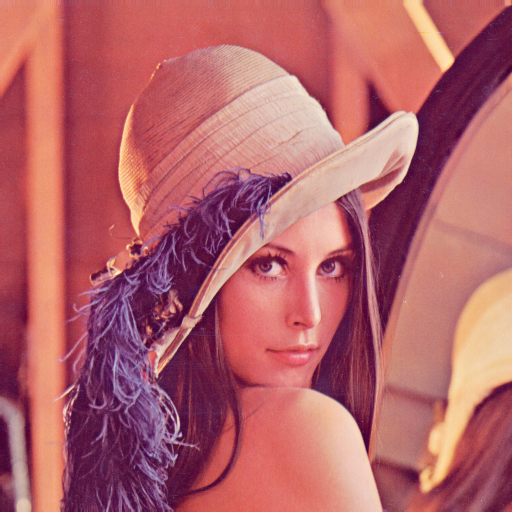
\includegraphics[width=.23\linewidth]{LennaRGB}}
\subcaptionbox{$\sigma = 1$}
  {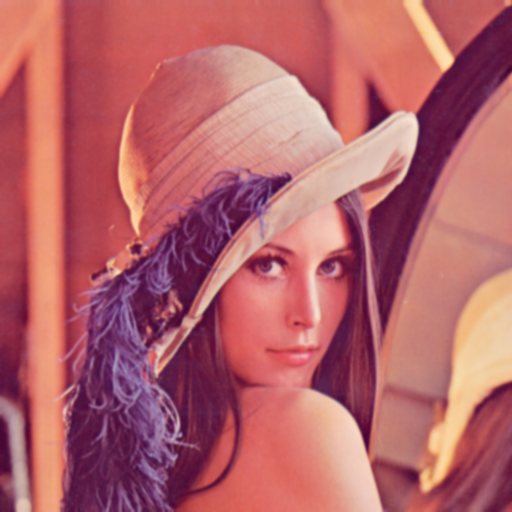
\includegraphics[width=.23\linewidth]{g1}}
\subcaptionbox{$\sigma = 5$}
  {
\includegraphics[width=.23\linewidth]{g2}}
\subcaptionbox{$\sigma = 10$}
  {
\includegraphics[width=.23\linewidth]{g3}}
\caption{Αποτελέσματα Canny για $thresh=0.2$}
\end{figure}
\newpage
\item \textbf{Gradient}

Η ακμή μίας εικόνας μπορεί να δείχνει σε διάφορες κατευθύνσεις, οπότε ο αλγόριθμος χρησιμοποιεί φίλτρα για να ανιχνεύσει  τις κάθετες και οριζόντιες ακμές στη θολή εικόνα. Ο τελεστής ανίχνευσης ακμών (Robers, Sobel ή Prewitt) επιστρέφει μια τιμή για την πρώτη παράγωγο στην οριζόντια κατεύθυνση - $G_x$ και στην κάθετη κατεύθυνση - $G_y$. Από τα δεδομένα αυτά μπορούμε να υπολογίσουμε το μέτρο της ακμής καθώς και την κατεύθυνσή της. Ο τελεστής χρησιμοποιεί δύο $3x3$ πυρήνες που συνελίσσονται με την εικόνα για να υπολογίσει προσεγγιστικά τις παραγώγους.
\[
  G_x=
  \begin{bmatrix}
     +1 & 0 & -1 \\
    +2 & 0 & -2 \\
    +1 & 0 & -1 \\
  \end{bmatrix}\quad
  G_y=
  \begin{bmatrix}
    +1 & +2 &+1 \\
    0 & 0 & 0 \\
    -1 & -2 & -1 \\
  \end{bmatrix}
\]

Ένας δεύτερος τρόπος για την εύρεση των ακμών είναι η απευθείας εύρεση των πρώτων παραγώγων χωρίς τη χρήση φίλτρων. Η κλίση μίας εικόνας $f(x,y)$ στην τοποθεσία $(x,y)$ μπορεί να οριστεί ως το διάνυσμα:

\begin{equation}
 \nabla(\boldsymbol{f}) = \begin{bmatrix}
    			 G_x \\
   				 G_y \\
  \end{bmatrix} =
  \begin{bmatrix}
    			 \frac{\partial f}{\partial x} \\
   				 \frac{\partial f}{\partial y} \\
  \end{bmatrix}
\end{equation}

\hfill \break
Και στις δύο περιπτώσεις το μέτρο και η κατεύθυνση της κλίσης υπολογίζεται με τη βοήθεια των ακόλουθων εξισώσεων:
\begin{equation}
G = \sqrt{G_x^2 + G_y^2}
\end{equation}
\begin{equation}
 \theta = \arctan{(G_y,G_x)}
\end{equation}
\item \textbf{Non-maximum suppression}

% http://www.cse.iitd.ernet.in/~pkalra/col783/canny.pdf

Η μέθοδος Non-maximum suppression είναι μία τεχνική αραίωσης της ακμής. Σκοπός αυτού του βήματος είναι η μετατροπή των `θολών' ακμών που ανιχνεύθηκαν σε `αιχμηρές'. Αυτό επιτυγχάνεται με τη διατήρηση όλων των τοπικών μεγίστων και τη διαγραφή όλων των άλλων. \\

\begin{itemize}
	\item Στρογγυλοποίηση της κατεύθυνσης της κλίσης στις πλησιέστερες 45 μοίρες, που αντιστοιχεί στη χρήση μια συνδεδεμένης γειτονιάς 8 εικονοστοιχείων
	\item Σύγκριση του μέτρου της κλίσης του τρέχοντος εικονοστοιχείου με το μέτρο του εικονοστοιχείου στην κατεύθυνση θετικής και αρνητικής κλίσης. Για παράδειγμα, εάν η κατεύθυνση της κλίσης είναι βόρεια ($\ang{90}$) τότε συγκρίνεται με τα εικονοστοιχεία προς το βορρά και το νότο
	\item Εάν το μέτρο του τρέχοντος εικονοστοιχείου είναι το μεγαλύτερο, διατηρείται η τιμή του, αλλιώς αφαιρείται. \\
\end{itemize}
\item \textbf{Κατωφλίωση}

Μετά την εφαρμογή της NMS, τα εναπομείναντα εικονοστοιχεία ακμών παρέχουν μία πιο ακριβή αναπαράσταση των πραγματικών ακμών της εικόνας. Ωστόσο, παραμένουν κάποιες ακμές που προκλήθηκαν από το θόρυβο και τις μεταβολές στο χρώμα της εικόνας. Προκειμένου να ληφθούν υπόψη οι ψευδείς αυτές απεικονίσεις, είναι απαραίτητο να φιλτραριστούν τα εικονοστοιχεία με αδύνατο μέτρο κλίσης και να διατηρηθούν αυτά που παρουσιάζουν υψηλή τιμή. Αυτό κατορθώνεται επιλέγοντας τιμές υψηλού και χαμηλού κατωφλίου.

Εάν το μέτρο κλίσης μιας ακμής είναι υψηλότερο από το υψηλό κατώφλι, σημειώνεται ως ακμή, αλλιώς εάν το μέτρο του είναι μικρότερο από το υψηλό κατώφλι και μεγαλύτερο από το χαμηλό κατώφλι σημειώνεται ως εικονοστοιχείο ασθενούς ακμής. Τέλος, αν η τιμή του μέτρου είναι μικρότερη από την τιμή του χαμηλού κατωφλίου, το εικονοστοιχείο καταστέλλεται. Οι δύο τιμές κατωφλίων καθορίζονται εμπειρικά και ο ορισμός τους θα εξαρτηθεί από το περιεχόμενο μιας δεδομένης εικόνας εισόδου. \\

\item \textbf{Ένωση ακμών με υστέρηση}

Μέχρι στιγμής, τα εικονοστοιχεία που έχουν κατηγοριοποιηθεί ως ισχυρές ακμές θα πρέπει σίγουρα να συμμετέχουν στην τελική εικόνα, καθώς έχουν προκύψει από τις πραγματικές ακμές της αρχικής εικόνας. Ωστόσο, θα πρέπει να παρθεί απόφαση σχετικά με τις ασθενείς ακμές που είναι πιθανό να έχουν προκύψει από θόρυβο. Για να επιτευχθεί, επομένως, ένα ακριβές αποτέλεσμα οι αδύναμες ακμές πρέπει να αφαιρεθούν.

Συνήθως ένα εικονοστοιχείο ασθενούς ακμής που προκαλείται από τις πραγματικές άκρες θα συνδέεται με μία ισχυρή ακμή. Για να συνδεθούν οι ακμές, μπορεί να εφαρμοστεί ανάλυση blob\footnote{https:\textbackslash\textbackslash en.wikipedia.org\textbackslash wiki\textbackslash Connected-component\_labeling} παρατηρώντας τα γειτονικά εικονοστοιχεία. Όσο υπάρχει μια ισχυρή ακμή που εμπλέκεται στην κηλίδα, αυτό το ασθενές άκρο μπορεί να αναγνωριστεί ως ένα που πρέπει να διατηρηθεί.

\end{itemize}

\subsection{Παραδείγματα εφαρμογής αλγορίθμου}

\begin{figure}[H]
\centering
\subcaptionbox{Είσοδος}%
  {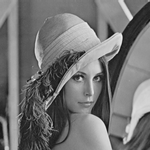
\includegraphics[width=.23\linewidth]{Lenna}}
\subcaptionbox{$\sigma = 1$}
  {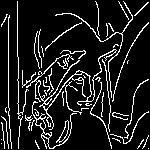
\includegraphics[width=.23\linewidth]{b1}}
\subcaptionbox{$\sigma = 5$}
  {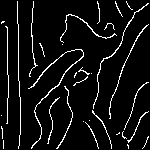
\includegraphics[width=.23\linewidth]{b2}}
\subcaptionbox{$\sigma = 10$}
  {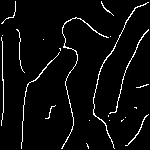
\includegraphics[width=.23\linewidth]{b3}}
\caption{Αποτελέσματα Canny για $thresh=0.2$}
\end{figure}
\begin{figure}[H]
\centering
\subcaptionbox{Είσοδος}%
  {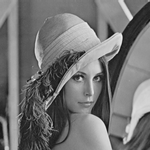
\includegraphics[width=.23\linewidth]{Lenna}}
\subcaptionbox{$\sigma = 1$}
  {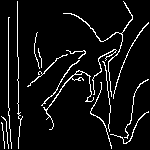
\includegraphics[width=.23\linewidth]{b4}}
\subcaptionbox{$\sigma = 5$}
  {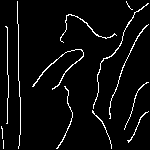
\includegraphics[width=.23\linewidth]{b5}}
\subcaptionbox{$\sigma = 10$}
  {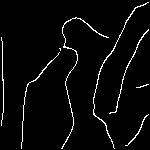
\includegraphics[width=.23\linewidth]{b6}}
\caption{Αποτελέσματα Canny για $thresh=0.5$}
\end{figure}

Παρατηρούμε ότι αυξάνοντας την τυπική απόκλιση του γκαουσιανού θολώματος, αρκετές σημαντικές ακμές της αρχικής εικόνας δεν αναγνωρίζονται. Αντίστοιχα, το ίδιο ισχύει και για το κατώφλι που έχουμε ορίσει. Στην πρώτη περίπτωση, το κατώφλι είναι κανονικοποιημένο ως προς το 255, δηλαδή ή κανονική τιμή του είναι $thresh=0.2\times 255=51$. Οι ακμές που έχουν τιμή μικρότερη του κατωφλίου απορρίπτονται. Στη δεύτερη περίπτωση, το κατώφλι είναι ίσο με $thresh=0.5\times 255=122.5$ και παρατηρούμε ότι αναγνωρίζονται πολύ λιγότερες ακμές.

Καταλήγοντας, πρέπει να οριστεί μία τιμή για την τυπική απόκλιση καθώς και μία για το κατώφλι, οι οποίες θα δίνουν σε σταθερή βάση ικανοποιητικά αποτελέσματα. Οι τιμές αυτές βρίσκοντας μετά από δοκιμές και εξαρτώνται συνήθως από τη φωτογραφία. Συνήθως, επιλέγουμε $\sigma=1.5$ και $thresh=45$.
